\HeaderQuote{There's a large mustard-mine near here. And the moral of that is -- The more there is of mine, the less there is of yours.}{The Duchess} 


\chapter{Evolutionary Learning of CDRs}\label{ch:esmodels} \todo[color=green!40,noline]{\cref{ch:esmodels} Unfinished, taken from GECCO submission}

%Evolutionary learning of weighted linear composite dispatching rules for scheduling

\FirstSentence{G}{enetic algorithms (GA) are one of the} most widely used approaches in \JSP\ literature \citep{Pinedo08}. However, in that case an extensive number of schedules need to be evaluated, and even for low dimensional \JSP\ that can quickly become computationally infeasible.
GAs can be used directly on schedules \citep{Cheng96,Cheng99,Tsai07,Qing-dao-er-ji12,Ak12,Meeran12}, however, in that case there are many concerns that need to be dealt with. To begin with there are nine encoding schemes for representing the schedules \cite{Cheng96}, in addition there has to be special care when applying cross-over and mutation operators in order for the schedules, now in the role of `chromosomes,' to still remain feasible. Moreover in case of \JSP\ the GAs are not adapt for fine-tuning around optima, luckily a subsequent local search can mediate the optimisation \citep{Cheng99,Meeran12}.

Another approach is to apply GAs indirectly to \JSP , via dispatching rules, i.e., Dispatching Rules Based Genetic Algorithms (DRGA) \citep{Vazquez-Rodriguez09,Dhingra10,Nguyen13} where a solution is no longer a \emph{proper} schedule but a \emph{representation} of a schedule via applying certain dispatching rules consecutively. 
DRGA are a special case of \emph{genetic programming} \citep{Koza05} which is the most predominant approach in hyper-heuristics is a framework of creating \emph{new} heuristics from a set of  predefined heuristics via GA optimisation \citep{Burke10}. 

A prevalent approach to solving \JSP\ is to combine several relatively simple dispatching rules such that they may benefit each other for a given problem space. Generally, this is done on an ad-hoc basis, requiring expert knowledge from heuristics designer, or extensive exploration of suitable combinations of heuristics. The approach in this \namecref{ch:esmodels}, is to automate that selection, by translating dispatching rules into measurable features and optimising what their contribution should be via evolutionary search. The framework is straight forward and easy to implement and shows promising results. Various data distributions from \cref{ch:genprobleminstances} are investigated, however only trained on the lower dimension, $6\times5$, yet, validated on higher dimension, $10\times10$. 

Moreover, \cref{sec:es:measure} shows that the choice of objective function  for evolutionary search is worth investigating. Since the optimisation is based on minimising the expected mean of the fitness function over a large set of problem instances, which can vary within. Then normalising the objective function can stabilise the optimisation process away from local minima. 

\section{Introduction}
As previously discussed in \cref{ch:introduction}, there are two main 
viewpoints on how to approach scheduling problems
\begin{enumerate*}
	\item local level by building schedules for one problem instance at a time
    \item global level by building schedules for all problem instances at once
\end{enumerate*}
{For local level construction a simple construction heuristic is applied, 
the schedule's features are collected at each dispatch iteration, from which a 
learning model will inspect the feature set to discriminate which operations 
are preferred to others via ordinal regression. The focus is essentially on 
creating a meaningful preference set composed of features and their ranks, as 
the learning algorithm is only run once to find suitable operators for the 
value function. This is the approach taken in \cref{InRu11a}.} 

Expanding on 
that  work, this study will explore global level construction viewpoint, where 
there is no feature set collected beforehand since the learning model is 
optimised directly via evolutionary search. This requires numerous costly value 
function evaluations. In fact it involves an indirect method of evaluation 
whether one learning model is preferable to another, w.r.t. which one yields a 
better expected mean. 



Inspired by DRGA, the approach taken in this study is to optimise the weights $\vec{w}$ in \cref{eq:jssp:linweights} directly, via evolutionary search such as covariance matrix adaptation evolution strategy (CMA-ES) \cite{Hansen01}, which has been proven to be a very efficient numerical optimisation technique. 

Using standard set-up of parameters of the CMA-ES optimisation, the runtime was limited to 288 hours on a cluster for each $6\times5$ training set given in \cref{sec:data:JSP,sec:data:FSP}, and in every case the optimisation reached its maximum walltime.

\section{Performance measures}\label{sec:es:measure}
Generally, evolutionary search only needs to minimise the expected fitness 
value, however the  approach in \cref{InRu11a} was to use the known optimum to 
correctly label which operations' features were indeed optimal compared to 
other possible operations, then it would be of interest to inspect if there is 
any performance edge gained in incorporating optimal labelling in evolutionary 
search. Therefore, two objective functions will be considered, namely, 
\begin{equation}
	ES_{C_{\max}} := \min \Exp[C_{\max}] \label{eq:cma:makespan}
\end{equation}
for optimising w.r.t. $C_{\max}$ directly, and on the other hand
\begin{equation}
	ES_{\rho} := \min \Exp[\rho] \label{eq:cma:rho}
\end{equation} 
which optimises w.r.t. the resulting $C_{\max}$ scaled to its true optimum, i.e., \cref{eq:rho}.

Main statistics of the experimental run are given in \cref{cma:funeval} and depicted in \cref{fig:cma:fit} for both approaches. In addition, evolving decision variables, here weights $\vec{w}$ for \cref{eq:jssp:linweights}, are depicted in \cref{fig:cma:wei}. 

In order to compare the two objective functions, the best weights reported were used for \cref{eq:jssp:linweights} on the corresponding training data. Its box-plot of percentage relative deviation from optimality, defined by \cref{eq:rho}, is depicted in \cref{fig:cma:trainboxpl} and main statistics detailed in \cref{tbl:results:train}. 

In the case of \frndn{6}{5}, \cref{eq:cma:rho}  gave a considerably worse results, since the optimisation got trapped in a local minimum, as the erratic evolution of the weighs in \cref{fig:cma:wei:cmax} suggest.
For other problem spaces, \cref{eq:cma:makespan} gave slightly better results than \cref{eq:cma:rho}, however, there was no statical difference between adopting either objective function. Therefore, minimisation of expectation of $\rho$, is preferred over simply using the unscaled resulting makespan. 

\begin{table}\centering
	\caption{Final results for CMA-ES optimisation.}\label{cma:funeval}
	\begin{tabular}{l |rrr |rrr}\toprule
		\multirow{2}{*}{$\mathcal{P}$}
		& \multicolumn{3}{c|}{minimise w.r.t. $C_{\max}$}& \multicolumn{3}{c}{minimise w.r.t. $\rho$} \\
		       & \#gen & \#eval & ES$_{C_{\max}}$ & \#gen & \#eval & ES$_\rho$ \\
		\midrule
		f.jc   & 5984  & 65835  & 567.688         & 1625  & 17886  & 0.361     \\
		f.rnd  & 5088  & 55979  & 571.394         & 4546  & 50006  & 7.479     \\
		f.rndn & 5557  & 61138  & 544.764         & 2701  & 29722  & 0.938     \\
		j.rnd  & 4707  & 51788  & 448.612         & 1944  & 21395  & 8.258     \\
		j.rndn & 4802  & 52833  & 449.942         & 1974  & 21725  & 8.691     \\
		\bottomrule
	\end{tabular}
\end{table}

\begin{figure}
	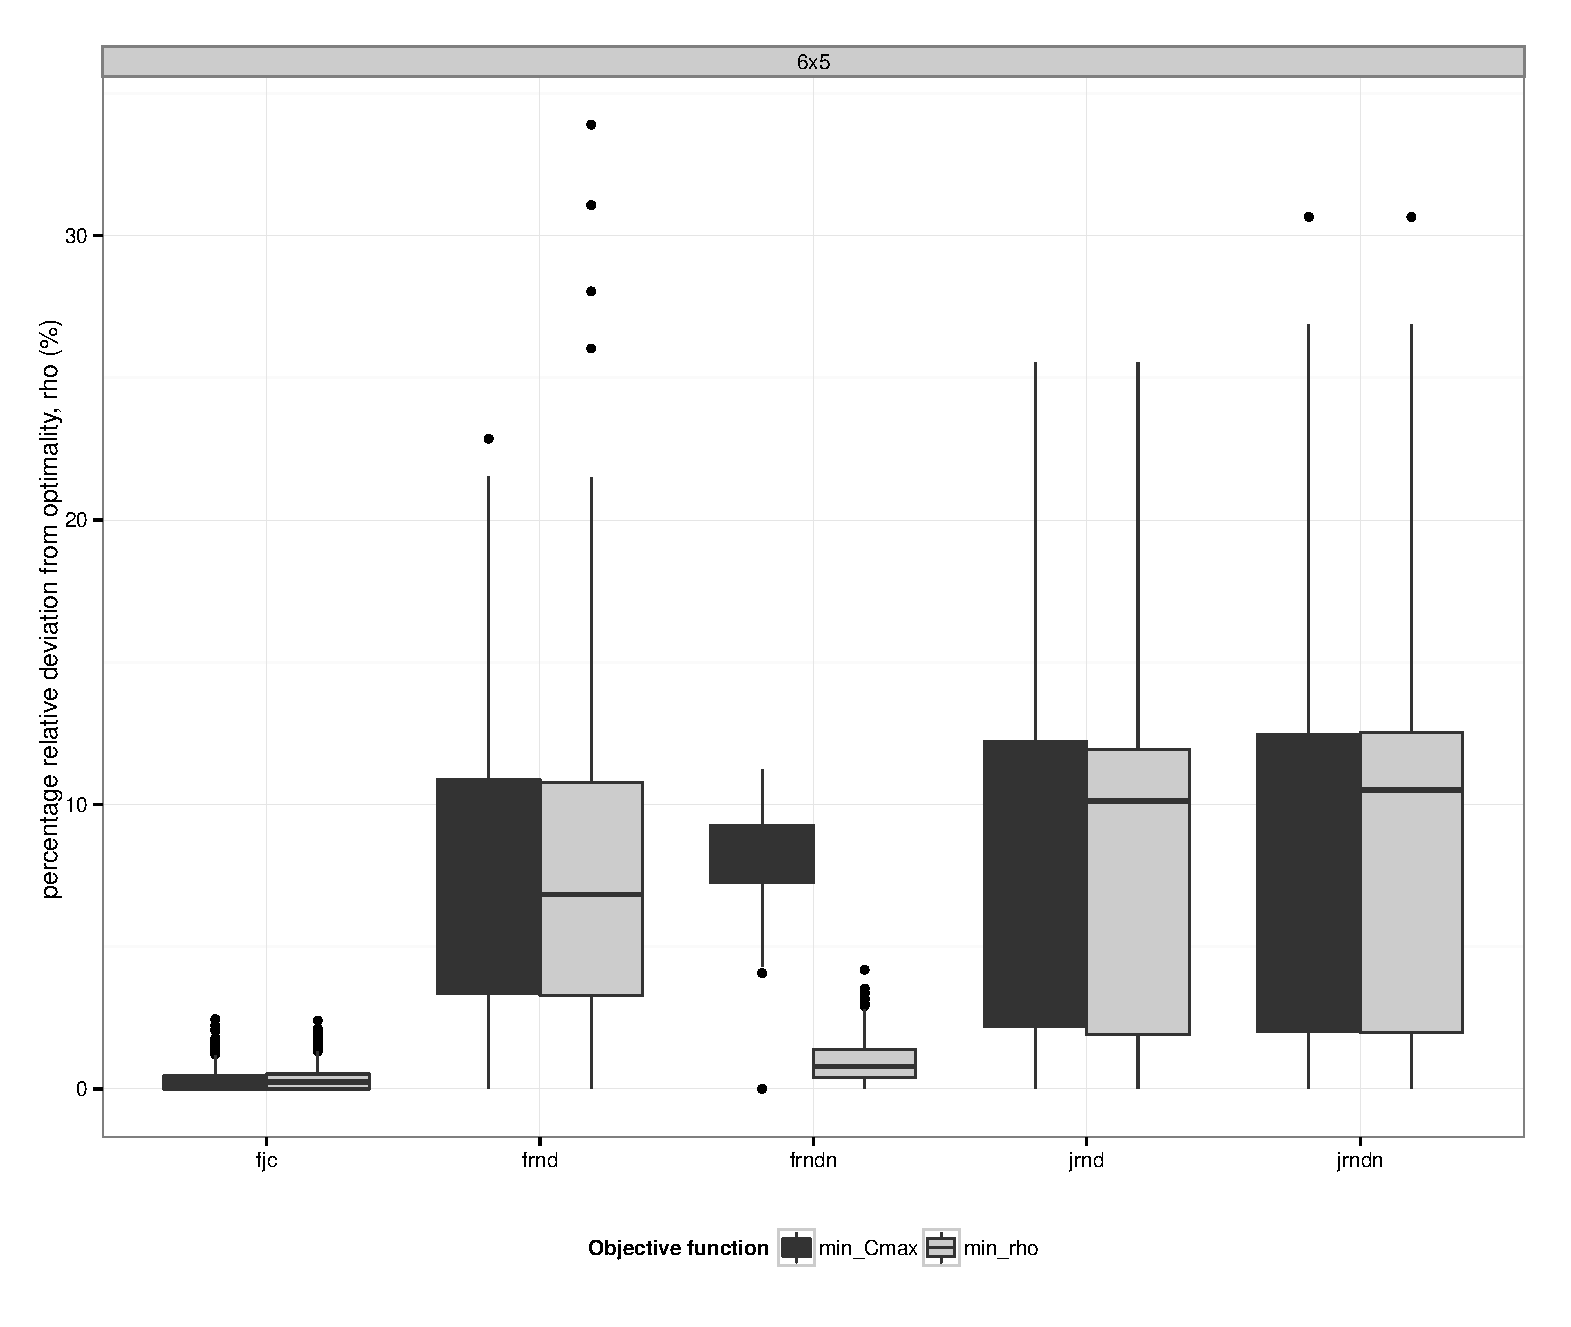
\includegraphics[width=\columnwidth]{CMAboxplotEvoTrain}
	\caption{Box-plot of training data for percentage relative deviation from optimality, defined by \cref{eq:rho}, when implementing the final weights obtained from CMA-ES optimisation, using both objective functions from \cref{eq:cma:makespan,eq:cma:rho}, left and right, respectively.}\label{fig:cma:trainboxpl}
\end{figure}

\subsection{Problem difficulty}\label{sec:expr:data}
The evolution of fitness per generation from the CMA-ES optimisation of \cref{eq:cma:rho} is depicted in \cref{fig:cma:fit}, and since all problem spaces reached their allotted computational time, without converging. In fact \frnd{6}{5} and \jrndn{6}{5} needed restarting during the optimisation process. 
Furthermore, the  evolution of the decision variables, $\vec{w}$, are depicted in \cref{fig:cma:wei}. As one can see, the relative contribution for each weight clearly differs between problem spaces. Note that in the case of \jrndn{6}{5} (cf. \cref{fig:cma:wei:rho}), CMA-ES restarts around generation 1,000 and quickly converges back to its previous fitness, however lateral relation of weights has completely changed. Implying that there are many optimal combinations of weights to be used, which can be expected due  to the fact some features in \cref{tbl:features} are a linear combination of one others, e.g., $\phi_3=\phi_1+\phi_2$.

\begin{figure} 
	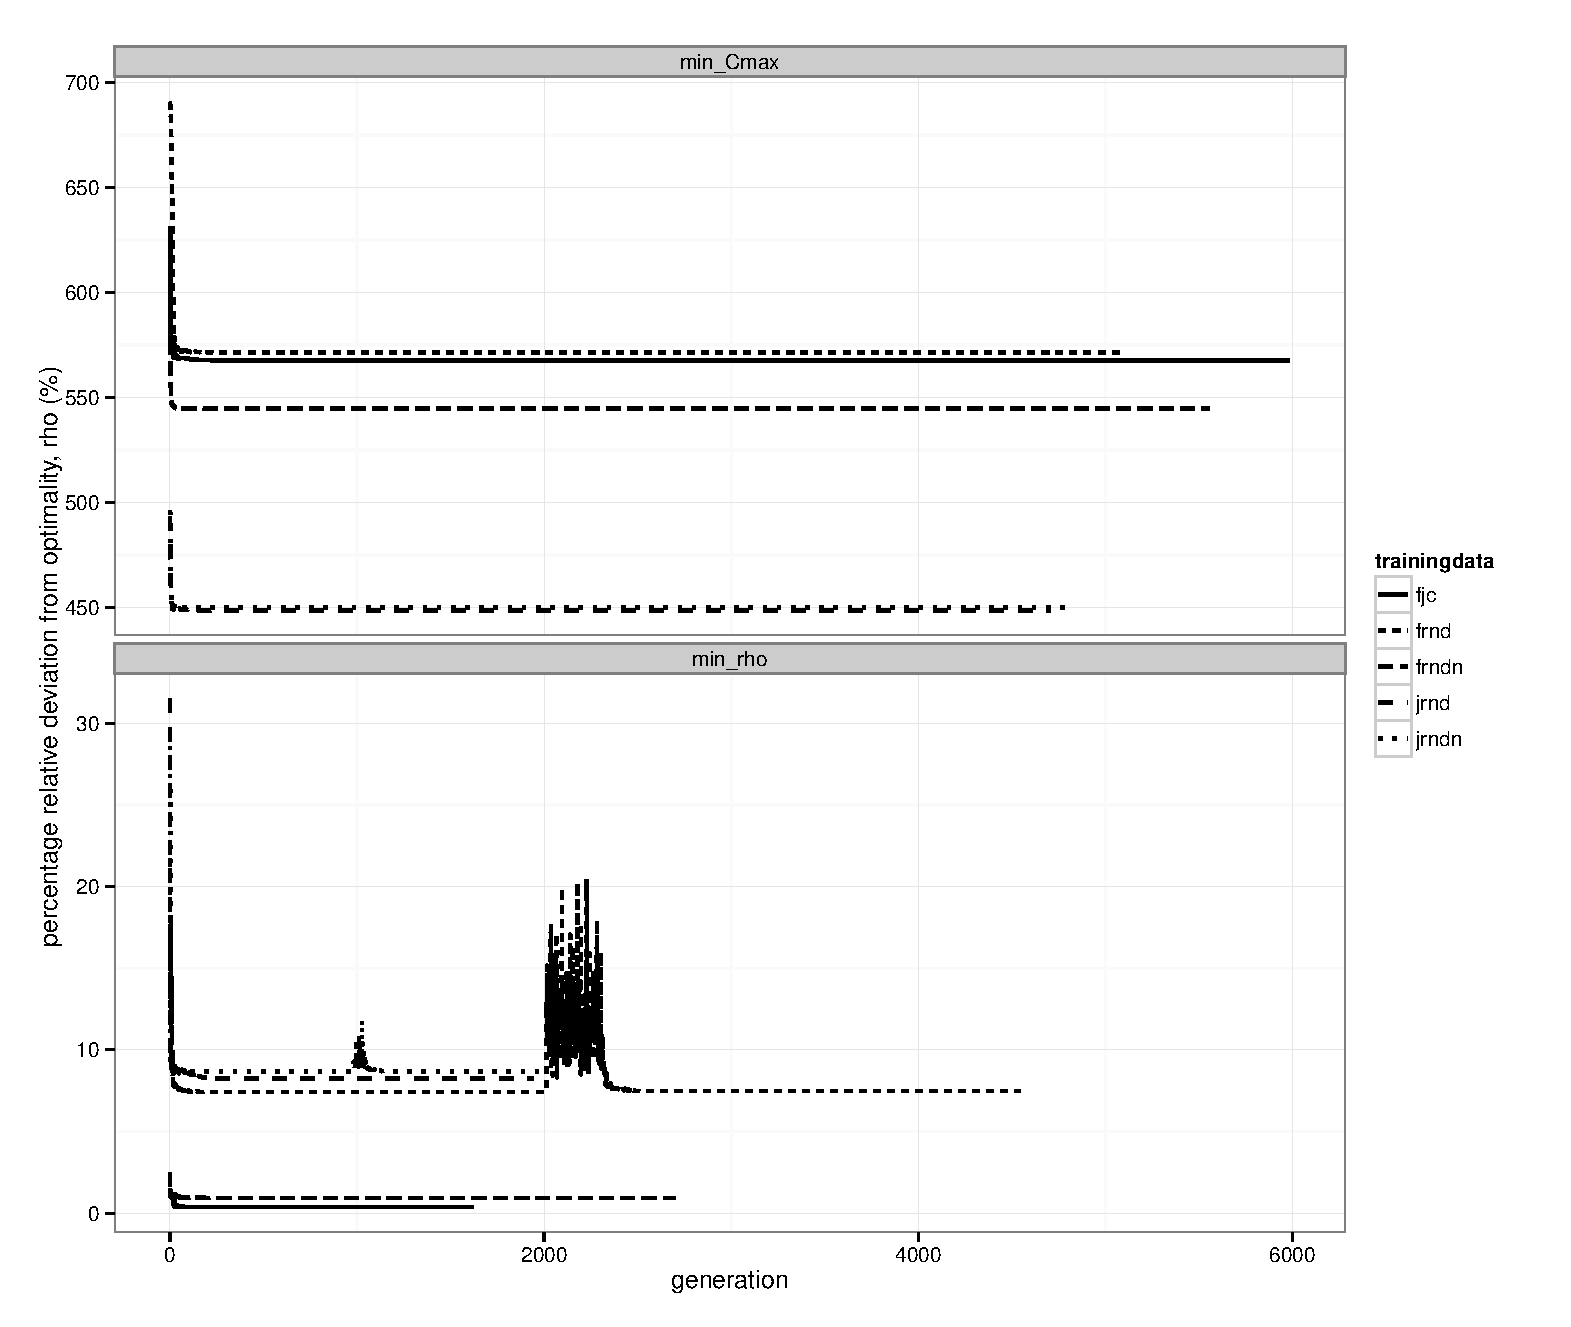
\includegraphics[width=\columnwidth]{CMAfitnessEvo}
	\caption{Fitness for optimising (w.r.t. \cref{eq:cma:makespan,eq:cma:rho} above and below, receptively), per generation of the CMA-ES optimisation.}\label{fig:cma:fit}
\end{figure}

\begin{figure*} 
	\subcaptionbox{minimise w.r.t. \cref{eq:cma:makespan}}{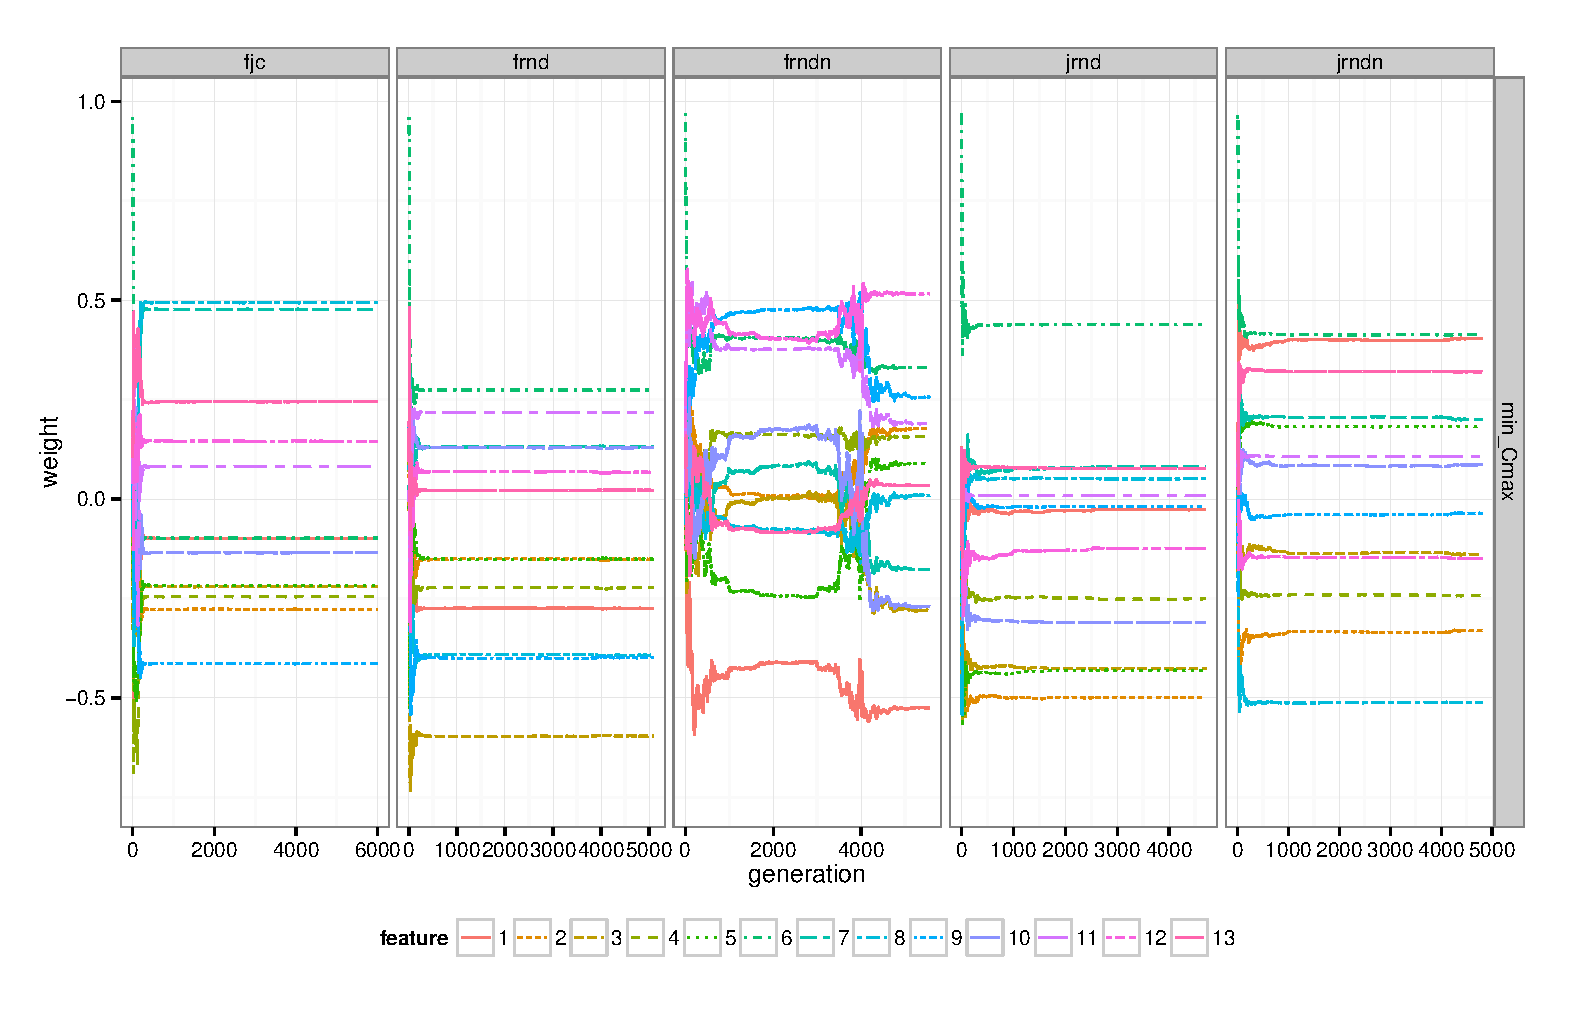
\includegraphics[width=\columnwidth]{CMAweightsEvomin_Cmax}\label{fig:cma:wei:cmax}}
	\\
	\subcaptionbox{minimise w.r.t. \cref{eq:cma:rho}}{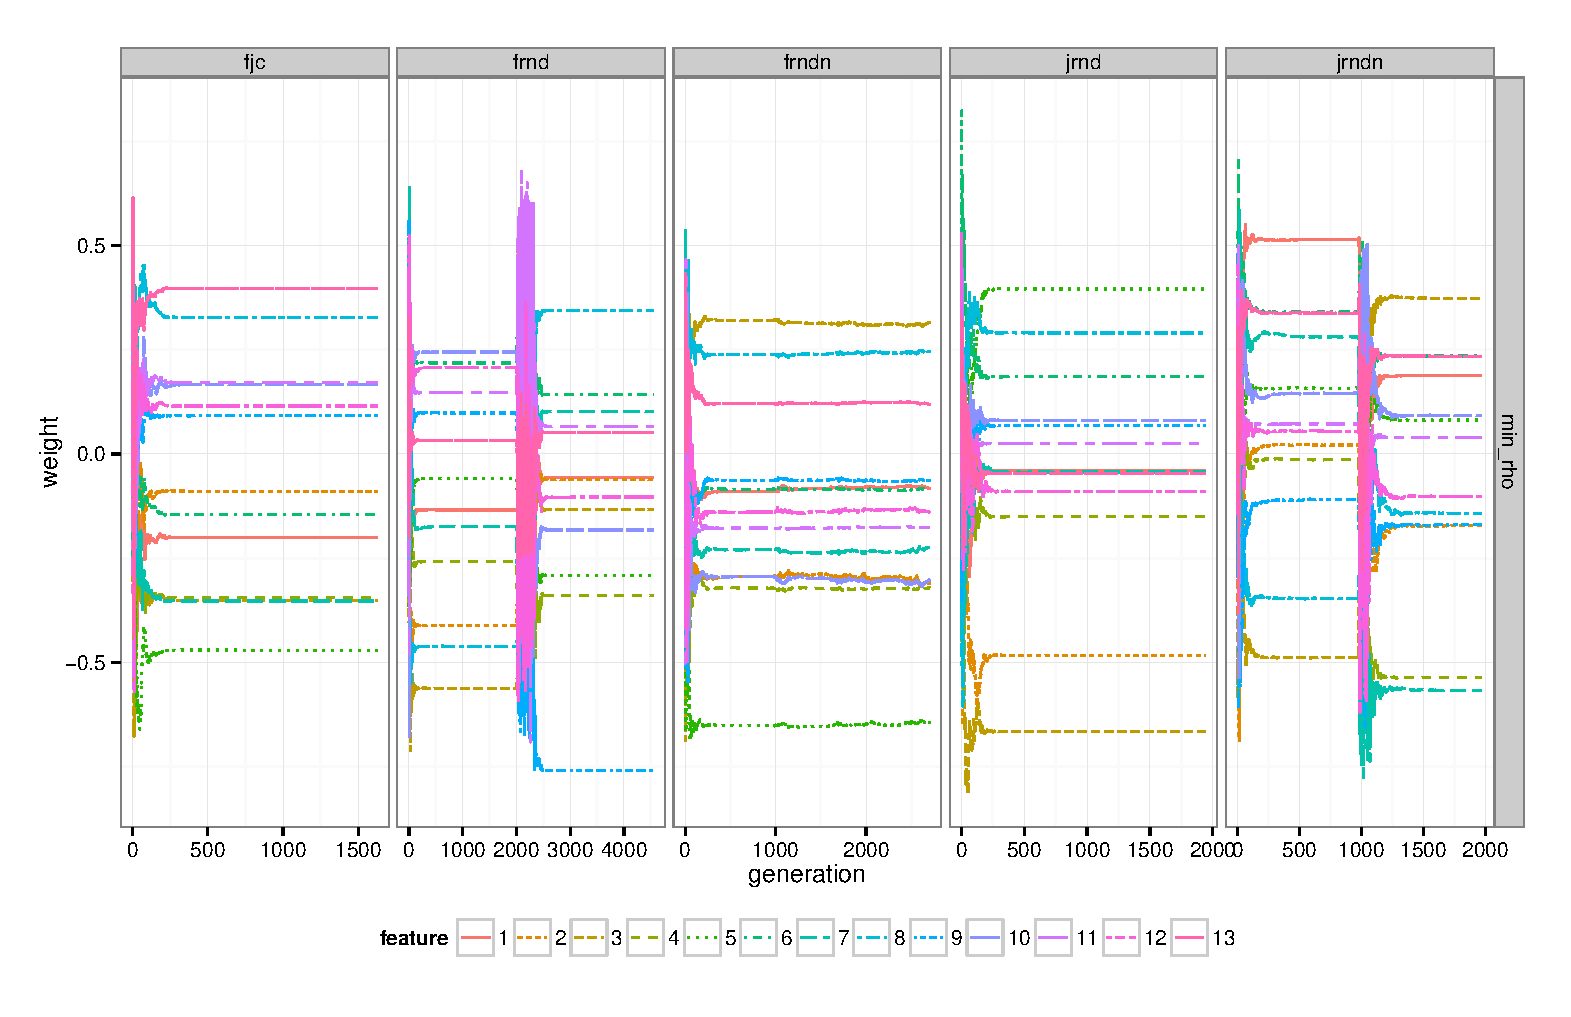
\includegraphics[width=\columnwidth]{CMAweightsEvomin_rho}\label{fig:cma:wei:rho}}
	\caption{Evolution of weights of features (given in \cref{tbl:features}) at each generation of the CMA-ES optimisation. Note, weights are normalised such that $\norm{\vec{w}}=1$.}\label{fig:cma:wei}
\end{figure*}


\subsection{Robustness and  scalability}\label{sec:expr:robust} 
As a benchmark, the linear ordinal regression model (PREF) from \cref{InRu11a} 
was created.
Using the weights obtained from optimising \cref{eq:cma:rho} and applying them on their  $6\times5$ training data, their main statistics of \cref{eq:rho} are reported in \cref{tbl:results:train}, for all training sets described in \cref{tbl:data}. Moreover, the best SDR, from which the features in \cref{tbl:features} were inspired by, are also reported for comparison, i.e., most work remaining (MWR) for all \JSP\ problem spaces, and least work remaining (LWR) for all \FSP\ problem spaces.

To explore the scalability of the learning methods, a similar comparison to \cref{sec:expr:robust} is made for the applying the learning models on their corresponding $10\times10$ testing data, results are reported in \cref{tbl:results:test}. Note that only resulting $C_{\max}$ is reported, as the optimum makespan is not known. 

{\setlength{\tabcolsep}{3pt}
	\begin{table}[p]\centering
\caption{Main statistics of percentage relative deviation from optimality, $\rho$, defined by \cref{eq:rho} for various models, using corresponding $6\times5$ training data.}
\label{tbl:results:train}
%jsp
\subfloat[][\jrnd{6}{5}]{\label{tbl:train:j.rnd}
\begin{tabular}{lrrrrr} \toprule
model&mean & med & sd & min & max \\   \midrule
ES$_{C_{\max}}$& 8.54 & 10 &  6 &  0 & 26   \\ % CMA-ES min_Cmax j.rnd 6x5 train
ES$_\rho$& 8.26 & 10 &  6 &  0 & 26   \\ % CMA-ES min_rho j.rnd 6x5 train
PREF&   10.18 & 11 &  7 &  0 & 30  \\ %PREF j.rnd 6x5 train
MWR &  16.48 & 16 &  9 &  0 & 45   \\ %MWR j.rnd 6x5 train
\bottomrule \end{tabular}}
\quad
\subfloat[][\jrndn{6}{5}]{\label{tbl:train:j.rndn}
\begin{tabular}{lrrrrr} \toprule
model&mean & med & sd & min & max \\   \midrule
ES$_{C_{\max}}$& 8.68 & 11 &  6 &  0 & 31   \\ % CMA-ES min_Cmax j.rndn 6x5 train
ES$_\rho$& 8.69 & 11 &  6 &  0 & 31   \\ % CMA-ES min_rho j.rndn 6x5 train
PREF&  10.00 & 11 &  6 &  0 & 31   \\ %PREF j.rndn 6x5 train
MWR &  14.02 & 13 &  8 &  0 & 37   \\ %MWR j.rndn 6x5 train
\bottomrule \end{tabular}}
\\
%flow shop
\subfloat[][\frnd{6}{5}]{\label{tbl:train:f.rnd}
\begin{tabular}{lrrrrr} \toprule
model&mean & med & sd & min & max \\   \midrule
ES$_{C_{\max}}$& 7.44 &  7 &  5 &  0 & 23   \\ % CMA-ES min_Cmax f.rnd 6x5 train
ES$_\rho$& 7.48 &  7 &  5 &  0 & 34   \\ % CMA-ES min_rho f.rnd 6x5 train
PREF&   9.87 &  9 &  7 &  0 & 38  \\ %PREF f.rnd 6x5 train
LWR &  20.05 & 19 & 10 &  0 & 71   \\ %LWR f.rnd 6x5 train
\bottomrule \end{tabular}}
\quad
\subfloat[][\frndn{6}{5}]{\label{tbl:train:f.rndn}
\begin{tabular}{lrrrrr} \toprule
model&mean & med & sd & min & max \\   \midrule
ES$_{C_{\max}}$& 8.09 &  8 &  2 &  0 & 11   \\ % CMA-ES min_Cmax f.rndn 6x5 train
ES$_\rho$& 0.94 &  1 &  1 &  0 &  4   \\ % CMA-ES min_rho f.rndn 6x5 train
PREF&   2.38 &  2 &  1 &  0 &  7  \\ %PREF f.rndn 6x5 train
LWR &  2.25 &  2 &  1 &  0 &  7   \\ %LWR f.rndn 6x5 train
\bottomrule \end{tabular}}
\\
\subfloat[][\fjc{6}{5}]{\label{tbl:train:f.jc}
\begin{tabular}{lrrrrr} \toprule
model&mean & med & sd & min & max \\   \midrule
ES$_{C_{\max}}$& 0.33 &  0 &  0 &  0 &  2   \\ % CMA-ES min_Cmax f.jc 6x5 train
ES$_\rho$& 0.36 &  0 &  0 &  0 &  2   \\ % CMA-ES min_rho f.jc 6x5 train
PREF&   1.08 &  1 &  1 &  0 &  5  \\ %PREF f.jc 6x5 train
LWR &  1.13 &  1 &  1 &  0 &  6   \\ %LWR f.jc 6x5 train
\bottomrule \end{tabular}}
\end{table}

	\begin{table}[p]\centering
\caption{Main statistics of $C_{\max}$ for various models, using corresponding $10\times 10$ test data.}
\label{tbl:results:test}
%jsp
\subcaptionbox{\jrnd{10}{10}}{\label{tbl:test:j.rnd}
\begin{tabular}{lrrrrr}  \toprule
model&mean & med & sd & min & max \\ 
  \midrule
ES$_{C_{\max}}$& 922.51 & 914 & 73 & 741 & 1173   \\ % CMA-ES min_Cmax j.rnd 10x10 test
ES$_\rho$& 931.37 & 931 & 71 & 735 & 1167   \\ % CMA-ES min_rho j.rnd 10x10 test
  PREF&   1011.38 & 1004 & 82 & 809 & 1281 \\   %PREF j.rnd 10x10 test
  MWR &  997.01 & 992 & 81 & 800 & 1273   \\ %MWR j.rnd 10x10 test
\bottomrule \end{tabular}}
\quad
\subcaptionbox{\jrndn{10}{10}}{\label{tbl:test:j.rndn}
\begin{tabular}{lrrrrr} \toprule
model& mean & med & sd & min & max \\ 
  \midrule
ES$_{C_{\max}}$& 855.85 & 857 & 50 & 719 & 1010   \\ % CMA-ES min_Cmax j.rndn 10x10 test
ES$_\rho$& 855.91 & 856 & 51 & 719 & 1020   \\ % CMA-ES min_rho j.rndn 10x10 test
  PREF&   899.94 & 898 & 56 & 769 & 1130  \\ %PREF j.rndn 10x10 test
  MWR&  897.39 & 898 & 56 & 765 & 1088   \\ %MWR j.rndn 10x10 test
\bottomrule \end{tabular}}
\\
%flow shop
\subcaptionbox{\frnd{10}{10}}{\label{tbl:test:f.rnd}
\begin{tabular}{lrrrrr} \toprule
model&mean & med & sd & min & max \\   \midrule
ES$_{C_{\max}}$& 1178.73 & 1176 & 80 & 976 & 1416   \\ % CMA-ES min_Cmax f.rnd 10x10 test
ES$_\rho$& 1181.91 & 1179 & 80 & 984 & 1404   \\ % CMA-ES min_rho f.rnd 10x10 test
PREF&  1215.20 & 1212 & 80 & 1006 & 1450  \\ %PREF f.rnd 10x10 test
LWR &  1284.41 & 1286 & 85 & 1042 & 1495   \\ %LWR f.rnd 10x10 test
\bottomrule \end{tabular}}
\quad 
\subcaptionbox{\frndn{10}{10}}{\label{tbl:test:f.rndn}
\begin{tabular}{lrrrrr} \toprule
model&mean & med & sd & min & max \\   \midrule
ES$_{C_{\max}}$& 1065.48 & 1059 & 32 & 992 & 1222   \\ % CMA-ES min_Cmax f.rndn 10x10 test
ES$_\rho$& 980.11 & 980 &  8 & 957 & 1006   \\ % CMA-ES min_rho f.rndn 10x10 test
PREF&  987.49 & 988 &  9 & 958 & 1011  \\ %PREF f.rndn 10x10 test
LWR &  986.94 & 987 &  9 & 959 & 1010   \\ %LWR f.rndn 10x10 test
\bottomrule \end{tabular}}
\\
\subcaptionbox{\fjc{10}{10}}{\label{tbl:test:f.jc}
\begin{tabular}{lrrrrr} \toprule
model&mean & med & sd & min & max \\   \midrule
ES$_{C_{\max}}$& 1135.44 & 1134 & 286 & 582 & 1681   \\ % CMA-ES min_Cmax f.jc 10x10 test
ES$_\rho$& 1135.47 & 1134 & 286 & 582 & 1681   \\ % CMA-ES min_rho f.jc 10x10 test
PREF&   1136.02 & 1135 & 286 & 582 & 1685 \\  %PREF f.jc 10x10 test
LWR &  1136.49 & 1141 & 287 & 581 & 1690   \\ %LWR f.jc 10x10 test
\bottomrule \end{tabular}}
\end{table}}

\section{Discussion and conclusions}\label{sec:disc}
Data distributions considered in this study either varied 
w.r.t. the processing times distributions, continuing the preliminary 
experiments in  \cref{InRu11a} , or 
w.r.t. the job ordering permutations, i.e., homogeneous $\sigma$ matrices in \FSP\ versus heterogeneous $\sigma$ matrices in \JSP . 
From the results based on $6\times5$ training data, given  in 
\cref{tbl:results:train}, it's obvious that CMA-ES optimisation substantially 
outperforms the previous PREF methods from \cref{InRu11a}, for all problem 
spaces considered. Furthermore, the results hold when testing on $10\times10$, 
(cf. \cref{tbl:results:test}), suggesting the method is indeed  scalable for 
higher dimensions. 

Moreover, the study showed that the choice of objective function  for 
evolutionary search is worth investigating. There was no statistical difference 
from minimising the fitness function directly and its normalisation w.r.t. true 
optimum (cf. \cref{eq:cma:makespan,eq:cma:rho}), save for \frndn{6}{5}. 
Implying, even though ES doesn't rely on optimal solutions, there are some 
problem spaces where it can be of great benefit. This is due to the fact that 
the problem instances can vary greatly within the same problem space 
\cref{InRu12}, thus normalising the objective function would help the 
evolutionary search to deviate the from giving too much weight for problematic 
problem instances for the greater good.

The weights for \cref{eq:jssp:linweights} in \cref{InRu11a} were found using 
supervised learning, where the training data was created from optimal solutions 
of randomly generated problem instances. As an alternative, this study showed  
that minimising the mean makespan directly using a brute force search via 
CMA-ES actually results in a better CDRs. The nature of CMA-ES is to explore 
suboptimal routes until it converges to an optimal one. Implying that the 
previous approach of only looking into one optimal route may not produce a 
sufficiently rich training set. That is, the training set should incorporate a 
more complete knowledge on \emph{all} possible preferences, i.e., make also the 
distinction between suboptimal and sub-suboptimal features, etc.  This would 
require a Pareto ranking of preferences which can be used to make the 
distinction to which feature sets are equivalent, better or worse -- and to 
what degree, i.e., by giving a weight to the preference. This would result in a 
very large training set, which of course could be re-sampled in order to make 
it computationally feasible to learn.

The main drawback of using evolutionary search for learning optimal weights for \cref{eq:jssp:linweights} is how computationally expensive it is to evaluate the mean expected fitness. Even for a low problem dimension, 6-job 5-machine \JSP , each optimisation run reached their walltime of 288hrs, without converging. Now, $6\times5$ \JSP\ requires 30 sequential dispatches, where at each time step there are up to $6$ jobs to choose from, i.e., its complexity is $\mathcal{O}(n^{n\cdot m})$, making it computationally infeasible to apply this framework for higher dimensions as is. 
However, evolutionary search only requires the rank of the candidates, and 
therefore it is appropriate to retain a sufficiently accurate surrogate for the 
value function during evolution in order to reduce the number of costly true 
value function evaluations, such as the approach in \cref{InRu11b}. This could 
reduce the computational cost of the evolutionary search considerably, making 
it feasible to conduct the experiments from \cref{sec:es:measure} for problems 
of higher dimensions, e.g., with these adjustments it is possible to train on 
$10\times10$ and test on for example $14\times14$ to verify whether scalability 
holds for even higher dimensions.  





